\documentclass[11pt]{article}
\usepackage[utf8]{inputenc}
\usepackage[T1]{fontenc}
\usepackage{amsmath,amssymb}
\usepackage{geometry}
\usepackage{listings}
\usepackage{xcolor}
\usepackage{hyperref}
\usepackage{tikz}
\usepackage{booktabs}
\usetikzlibrary{calc, arrows.meta, positioning}

\geometry{margin=2.5cm}

\lstdefinelanguage{Rust}{
  keywords={fn,let,mut,for,in,if,else,while,loop,match,return,struct,impl,pub,use,mod,as,where,move,ref,self,Self,crate,super,async,await,unsafe,const,static,type,enum,trait, dyn, true, false, continue, break},
  keywordstyle=\color{blue!70!black}\bfseries,
  ndkeywords={Vec,Vec3,Mat4,Mesh,MeshVertex,SceneNode,Scene,PbrMaterial,Affine3A,u32,usize,f32,f64,bool,Option,Some,None,Result,Ok,Err,String},
  ndkeywordstyle=\color{purple!70!black}\bfseries,
  sensitive=true,
  comment=[l]{//},
  morecomment=[s]{/*}{*/},
  commentstyle=\color{green!50!black}\itshape,
  stringstyle=\color{red!70!black},
  morestring=[b]",
}

\lstset{
  basicstyle=\ttfamily\footnotesize,
  breaklines=true,
  frame=single,
  language=Rust,
  showstringspaces=false,
  tabsize=2,
}

\title{Bounding Wireframes for Implicit Surfaces:\\
       Cube and Sphere Outlines via Selective Edge Overlay}
\author{engvis}
\date{\today}

\begin{document}
\maketitle

\section{Problem Statement}

The \texttt{engvis} viewer renders implicit surfaces $\{f=0\}$
restricted to a working domain $\Omega$:
\begin{itemize}
  \item \texttt{gyroid}: $\Omega = [-1,1]^3$ (cube)
  \item \texttt{gyroid-sphere}: $\Omega = \{\mathbf{p}\in\mathbb{R}^3 :
        \|\mathbf{p}\|\le R\}$ (ball, $R=1$)
\end{itemize}

When the surface is open (its boundary lies on $\partial\Omega$), the
viewer needs a visual cue showing \emph{which} domain the surface lives
in.  Without this cue, the eye cannot tell whether a curved silhouette
is a feature of $f$ or merely the clip against $\partial\Omega$.

We add a wireframe outline of $\partial\Omega$ rendered as line
segments, so $\Omega$ is unambiguous while the lit surface itself stays
free of triangle-edge clutter.

\section{Design Choices}

\subsection{Why selective edge overlay, not a separate line shader}

\texttt{engvis} already has a triangle-line pipeline in
\texttt{OverlayRenderer} that turns each mesh edge $(A,B)$ into a quad
of constant pixel width.  Hooking the bounding outline into this
pipeline avoids introducing a parallel line shader and reuses the
MSAA / depth state set up for the rest of the frame.

The edge overlay, however, was written to draw \emph{every} triangle
edge of \emph{every} mesh.  Drawing every edge of the gyroid surface
(\(\sim10^4\) triangles) would bury the bounding outline.  We
therefore introduce a per-node opt-in flag, so only the wireframe
mesh contributes to the edge pass:

\begin{lstlisting}
pub struct SceneNode {
    // ...
    /// Whether to draw this node's edges in the edge-overlay pass.
    pub render_edges: bool,
}
\end{lstlisting}

In the renderer:

\begin{lstlisting}
let skip_mesh = matches!(mode, OverlayDrawMode::Edges)
                && !node.render_edges;
if !skip_mesh && let Some(mesh_idx) = node.mesh_index { ... }
\end{lstlisting}

\subsection{Why degenerate triangles, not a dedicated line mesh}

The mesh data structure \texttt{Mesh} stores triangles in
\texttt{indices: Vec<u32>}.  Adding a separate ``line list'' channel
would force every downstream pass (vertex extraction, AABB, GPU upload)
to carry two parallel buffers.

We instead encode each line segment $(A,B)$ as a \emph{degenerate
triangle} $(A, B, A)$.  This works because:
\begin{itemize}
  \item \texttt{extract\_edge\_indices()} unpacks each triangle
        $(i_0,i_1,i_2)$ into edges $(i_0,i_1), (i_1,i_2), (i_2,i_0)$,
        which for $(A,B,A)$ becomes $(A,B), (B,A), (A,A)$.  The first
        two are the same line in opposite directions; the third has
        zero length and contributes a zero-area quad.
  \item In the PBR rasterisation pass the triangle has zero area, so
        no fragments are produced --- the wireframe never appears as
        a solid surface.
\end{itemize}

\section{Geometry}

\subsection{Cube wireframe (gyroid)}

The cube $[-1,1]^3$ has $8$ corners $V_i$ and $12$ edges
$E_k = (V_{a_k}, V_{b_k})$.  Each edge $E_k$ becomes a degenerate
triangle in the mesh:
\[
  \texttt{indices} \mathrel{+}= [\, 2k,\; 2k+1,\; 2k\,].
\]

\subsection{Sphere wireframe (gyroid-sphere)}

The sphere of radius $R=1$ is approximated by a latitude--longitude
grid.  With $n_\text{lat}=12$, $n_\text{lon}=24$ we generate
\begin{itemize}
  \item $n_\text{lon}$ \emph{meridians}, each subdivided into
        $2n_\text{lat}$ polar arcs:
        \[
          \mathbf{p}(\varphi, \theta) =
          R\,(\sin\theta\cos\varphi,\; \cos\theta,\; \sin\theta\sin\varphi),
          \quad
          \theta \in [0,\pi],\;
          \varphi = \tfrac{2\pi i}{n_\text{lon}}.
        \]
  \item $n_\text{lat}-1$ \emph{parallels}, each subdivided into
        $2n_\text{lat}$ azimuthal arcs:
        \[
          \mathbf{p}(\varphi)
          = (R\sin\theta_j\cos\varphi,\; R\cos\theta_j,\;
             R\sin\theta_j\sin\varphi),
          \quad
          \theta_j = \tfrac{\pi j}{n_\text{lat}}.
        \]
\end{itemize}
Total segment count: $n_\text{lon}\cdot 2n_\text{lat}
+ (n_\text{lat}-1)\cdot 2n_\text{lat}$
$= 2n_\text{lat}(n_\text{lon}+n_\text{lat}-1)$,
which for $(12,24)$ gives $840$ segments.

\section{Pipeline}

\begin{figure}[h]
  \centering
  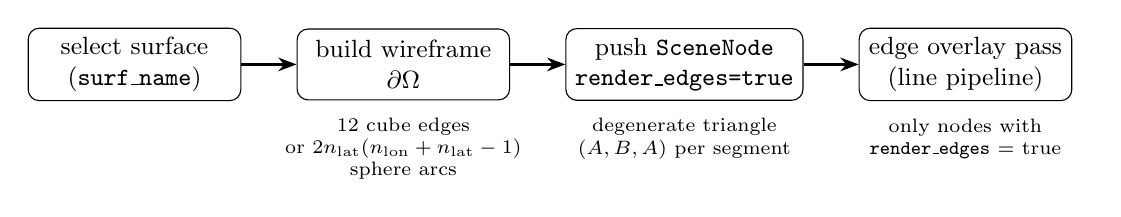
\begin{tikzpicture}[
      node distance=6mm and 7mm,
      box/.style={draw, rounded corners, align=center, minimum height=9mm,
                  minimum width=27mm, font=\small},
      arr/.style={-Stealth, thick}
    ]
    \node[box] (sel)  {select surface\\(\texttt{surf\_name})};
    \node[box, right=of sel] (wf)
      {build wireframe\\$\partial\Omega$};
    \node[box, right=of wf] (node)
      {push \texttt{SceneNode}\\\texttt{render\_edges=true}};
    \node[box, right=of node] (pass)
      {edge overlay pass\\(line pipeline)};

    \draw[arr] (sel) -- (wf);
    \draw[arr] (wf)  -- (node);
    \draw[arr] (node)-- (pass);

    \node[below=1mm of wf, font=\scriptsize, text width=30mm, align=center]
      {12 cube edges\\or $2n_\text{lat}(n_\text{lon}+n_\text{lat}-1)$\\sphere arcs};
    \node[below=1mm of node, font=\scriptsize, text width=32mm, align=center]
      {degenerate triangle\\$(A,B,A)$ per segment};
    \node[below=1mm of pass, font=\scriptsize, text width=30mm, align=center]
      {only nodes with\\\texttt{render\_edges} = true};
  \end{tikzpicture}
  \caption{\label{fig:flow} Wireframe construction and selective
    edge-overlay pass.  The PBR pass ignores the wireframe mesh
    because every triangle has zero area; the edge pass ignores
    every other node because they have \texttt{render\_edges = false}.}
\end{figure}

\section{Comparison}

\begin{table}[h]
  \centering
  \begin{tabular}{lcc}
    \toprule
    Approach & Reuses overlay pipeline? & Per-node control? \\
    \midrule
    New line shader               & no  & n/a  \\
    Edge overlay, all meshes      & yes & no   \\
    Edge overlay, \texttt{render\_edges} flag & yes & \textbf{yes} \\
    \bottomrule
  \end{tabular}
  \caption{Trade-offs of bounding-outline rendering strategies.  The
    chosen approach is the only one that reuses the existing pipeline
    \emph{and} keeps the surface mesh's triangle edges hidden.}
\end{table}

\section{Implementation Summary}

\begin{itemize}
  \item \texttt{src/main.rs}
        \begin{itemize}
          \item \texttt{build\_box\_wireframe()} --- 12-edge cube outline.
          \item \texttt{build\_sphere\_wireframe(r, n\_lat, n\_lon)} ---
                lat/lon sphere outline.
          \item In \texttt{App::build\_scene()}: choose
                cube / sphere wireframe by \texttt{surf\_name}, push as
                an extra node with \texttt{render\_edges = true}.
          \item In \texttt{App::ui()}: enable
                \texttt{frame.render\_state.edge\_opts}
                (colour, line width).
          \item \texttt{clip\_mesh\_to\_ball(.., r=1.0)}: clipping ball
                radius now matches the wireframe.
        \end{itemize}
  \item \texttt{crates/engvis-core/src/scene.rs}: add
        \texttt{render\_edges: bool} field to \texttt{SceneNode} (default
        \texttt{false} in \texttt{Scene::single\_mesh}).
  \item \texttt{crates/engvis-renderer/src/renderer.rs}: in
        \texttt{render\_overlay\_node}, skip nodes with
        \texttt{render\_edges = false} when \texttt{mode = Edges}.
  \item \texttt{crates/engvis-renderer/src/gltf\_loader.rs}: initialise
        \texttt{render\_edges = false} for imported nodes.
\end{itemize}

\section{Result}

\begin{itemize}
  \item \texttt{gyroid}: a thin cube outline
        $[-1,1]^3$ frames the lit gyroid mesh; the surface itself shows
        no triangle edges.
  \item \texttt{gyroid-sphere}: the lat/lon sphere ($R=1$) frames the
        spherically-clipped gyroid patch.  The surface boundary lies
        exactly on this sphere because \texttt{clip\_mesh\_to\_ball}
        cuts at the same radius.
  \item Both outlines respect MSAA, depth, and the configurable line
        width / colour from \texttt{EdgeRenderOptions}, with no extra
        shader code.
\end{itemize}

\end{document}
